The Integer Factorization problem is defined as follows; given a composite integer $n$, find any non-trivial factor $e$ of $n$, such that $e|n$. At first it might seem like a trivial task, but for large integers this has proven to be a very difficult task.

\subsection{Trial Division}
 The most straight-forward approach to factoring composite numbers is \emph{trail division}, which essentially (just like its name suggests) just check for every prime number $p \leq \sqrt{n}$ if $p|n$. 

Improvement is to only do tests when $p$ is a prime number, i.e. keep a list of precomputed prime numbers. Although trial division is easy to implement and guaranteed to grant an answer it is not efficient with large integers. There is improvements that can be applied such as storing a precomputed tables of primes to bring up the speed. However, this instead requires alot of memory during run-time as well as storage, when dealing with larger integers. A

\subsection{Pollard's $\rho$}
In 1975 John M. Pollard proposed a new and very efficient Monte Carlo algorithm for factoring integers, now known as Pollard's $\rho$ (rho) method.
It was a break through and proved to be alot more faster than its predecessor trial division for finding small non-trivial factors of a large integer $n$.

\subsubsection{Basic idea}
Pollard's $p$ basic concept is that a sequence of pseudo-random integers constructed as

\begin{equation}
x_0 = \texttt{rand}(0,\ n-1) 
\end{equation}

\begin{equation}
x_i = f(x_{i-1}) \ (\texttt{mod} \ n), \ \texttt{for} \ i = 1, 2, \ldots
\end{equation}

where $f$ is polynomial which in most practical implementations has the form $f(x) = x^2 + \alpha, \alpha \neq 0, -2$.
The key observation that if we consider a non-trivial divisor of $n$, say $d$, that is small compared to $n$. Then there exists smaller congruence
groups modulo $d$ compared to $n$. Because of this there is a probability that there exists two $x_i$ and $x_j$ such that $x_i \equiv x_j$ (mod $d$),
while $x_i \not\equiv x_j$ (mod $n$). Thus it follows from that gcd$(x_i - x_j, n)$ is a non-trivial factor of $n$.

The idea of pollard rho algorithm is to iterate a formula until it falls into a cycle. We want to find a $x$ and $y$ whereas the $x$ makes twice as many iterations as the $y$ using a function (mod $n$) as a generator of a pseudo-random sequence. The $gcd(x - y, n)$ is taken each step, and it reaches $n$ we have not found an answer and the algorithm terminates with a failure.

We can write $n = p \cdot q$, when $x$, which iterates twice as fast as $y$, catches up with $y$ which will happen eventually, at this point factor $p$ will be found. The time it will take cannot be proven matematically and can only be proven by heuristics. If the sequence behaves randomly it would take approximately p steps to find p, which is not very effcient. \cite{avalg} 

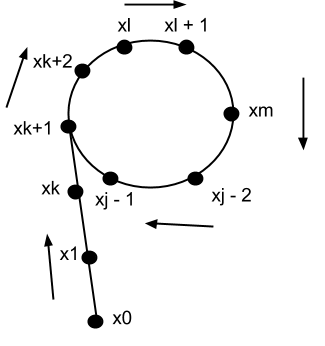
\includegraphics[scale = 0.5]{pollards.png}

The figure above illustrates the Pollard's Rho cycle. The mapping of $x_{i+1}$ is instead replaced with a function $x^2+1$ so that we get $x^2_{i}+1$  $mod$ $N$ the factor $p$ will be found after $O(\sqrt{p})$  $\epsilon$ $O(N^{1/4})$ steps. \cite{avalg}\\

Pollard's rho algorithm can be improved further by implementing Brent's cycle finding method. \cite{brent}

\subsection{Miller-Rabin primality test}
Miller-Rabin primality test is a probabalistics algorithm which determines if the given input $N$ is a prime. It is based on the properties of strong pseudoprimes, given an integer $N$, $N = 2^r * s + 1$ where $s$ is odd, you choose a random number $a$ with the properties $1 \leq a \leq N - 1$. When $a^s \equiv 1$ $mod$ $N$ or $a^{2js} \equiv - 1$ $mod$ $N$ where $0 \leq j \leq r - 1$, if the input number $N$ is a prime it will pass the test with any random number $a$.

Since Miller-Rabin is a probabalistics method it is not completely true that $N$ is a prime simply by passing the test, however the probability that the answer is true when $N$ is a composite number is $1 / 4^{N}$ which grows quickly with $N$. It can be considered a very small trade-off to use a probabalistics method because the algorithm executes at $O(k$ $log^3 N)$ where $k$ is the number of different values of $a$ tested. \cite{miller}
